\documentclass{article}
%Usepackages
\usepackage{adjustbox, amsmath, amssymb, amsthm, blindtext, bm, bbm, dblfloatfix, esint, fancyhdr, float, graphicx, letltxmacro, marginnote, mathtools, subcaption, xcolor, titlesec, esint}
\usepackage{amssymb}
\usepackage[font={small, it}]{caption}
\usepackage{amsmath}
\usepackage{floatrow}
\usepackage{times}
\usepackage{ stmaryrd }
\usepackage{amsthm}
\usepackage{xcolor}
\usepackage{mathrsfs}
\usepackage[colorlinks = true,
            linkcolor = black,
            urlcolor  = blue,
            citecolor = black,
            anchorcolor = blue]{hyperref}
% \usepackage[mathscr]{euscript}
\usepackage{mathrsfs}
\usepackage{wasysym}
%\usepackage{pxfonts}
\usepackage[letterpaper, portrait, margin=1in]{geometry}
\usepackage{graphicx}
\usepackage{tikz}
\usepackage{tikz-3dplot}
\usepackage{pgfplots}
\usetikzlibrary{decorations.pathmorphing,patterns}
\usepackage{lipsum}
\usepackage{float}
\usepackage{subcaption}
\usepackage[object=vectorian]{pgfornament}
\usepackage{mwe}
\usepackage{bigints}
\usepackage{csquotes}
\usepackage{titlesec}
\usepackage{halloweenmath}
\setcounter{secnumdepth}{4}
\titleformat{\paragraph}
{\normalfont\normalsize\bfseries}{\theparagraph}{1em}{}
\titlespacing*{\paragraph}
{0pt}{3.25ex plus 1ex minus .2ex}{1.5ex plus .2ex}
\usepackage{mathtools}
\usepackage{pgfplots}
\pgfplotsset{compat=1.15}
\usepackage{lastpage}
\usepackage{enumitem}
\usepackage{tensor}
\usepackage{mathtools}

% This is for the header:
% https://tex.stackexchange.com/questions/75168/get-current-section-name-without-label
\usepackage{nameref}
\makeatletter
\newcommand*{\currentname}{\@currentlabelname}
\makeatother

\usepackage{fancyhdr} 
    \pagestyle{fancy}
    \fancyhf{}
    \fancyhead[R]{ Page \thepage \  of \pageref{LastPage}}
    \fancyhead[L]{\currentname}
\usepackage{setspace}
\usepackage{tikz}
\usetikzlibrary{hobby}

\usepackage{pst-node}
\usepackage{tikz-cd}
\usepackage[most]{tcolorbox}

% \makeatletter
% \renewcommand\@endtheorem{\vvv@endmarker\endtrivlist\@endpefalse}
% \newcommand\vvv@endmarker{%
%   {\unskip\nobreak\hfil\penalty50
%   \hskip2em\vadjust{}\nobreak\hfil\openbox
%   \parfillskip=0pt \finalhyphendemerits=0 \par
%   \penalty 10000 \parskip=0pt\noindent}\ignorespaces}
% \makeatother

\theoremstyle{definition}

% https://tex.stackexchange.com/questions/616586/how-to-make-a-tcolorbox-with-only-a-left-side-rule


\newtheorem{thm}{Theorem}[section]
\newtheorem{defn}[thm]{Definition}
\newtheorem{exmp}[thm]{Example}
\newtheorem{lem}[thm]{Lemma}
\newtheorem{conjecture}[thm]{Conjecture}
\newtheorem{exercise}[thm]{Exercise}
\newtheorem{fact}[thm]{Fact}
\newtheorem{claim}[thm]{Claim}
\newtheorem{cor}[thm]{Corollary}
\newtheorem{summary}[thm]{Summary}

\newtheorem{idea}[thm]{Idea}
\newtheorem{application}[thm]{Application}
\newtheorem{rmk}[thm]{Remark}

\newtheorem{prop}[thm]{Proposition}
\newtheorem{ques}[thm]{Question}

\newtcolorbox{cbox}[1][]{
            breakable,
            boxrule=0pt,
            frame hidden,
            sharp corners,
            enhanced,
            borderline west={2pt}{0pt}{#1},
            colback=#1!5!white}

% \newenvironment{cthm}[3]
%     {\begin{cbox}[#2]
%     \color{#2}
%     \begin{#3}[#1]
%     \color{black}
%     }
%     {
%     \end{#3} 
%     \end{cbox}
%     }

% \newenvironment{theorem}[1][]
% {\begin{cthm}{#1}{orange}{thm}}
% {\end{cthm}}

\newenvironment{theorem}[1][]
    {\begin{cbox}[blue]
    \color{blue}
    \begin{thm}[#1]
    \color{black}
    }
    {
    \end{thm} 
    \end{cbox}
    }

\newenvironment{corollary}[1][]
    {\begin{cbox}[orange]
    \color{orange}
    \begin{cor}[#1]
    \color{black}
    }
    {
    \end{cor} 
    \end{cbox}
    }

\newenvironment{lemma}[1][]
    {\begin{cbox}[orange]
    \color{orange}
    \begin{lem}[#1]
    \color{black}
    }
    {
    \end{lem} 
    \end{cbox}
    }

\newenvironment{proposition}[1][]
    {\begin{cbox}[orange]
    \color{orange}
    \begin{prop}[#1]
    \color{black}
    }
    {
    \end{prop} 
    \end{cbox}
    }

\newenvironment{definition}[1][]
    {\begin{cbox}[red]
    \color{red}
    \begin{defn}[#1]
    \color{black}
    }
    {
    \end{defn} 
    \end{cbox}
    }

\newenvironment{example}[1][]
    {\begin{cbox}[violet]
    \color{violet}
    \begin{exmp}[#1] \color{black}
    }
    {
    \end{exmp} 
    \end{cbox}
    }

\newenvironment{question}[1][]
    {\begin{cbox}[black]
    \begin{ques}[#1]
    }
    {
    \end{ques} 
    \end{cbox}
    }

\newenvironment{remark}[1][]
    {\begin{cbox}[black]
    \begin{rmk}[#1]
    }
    {
    \end{rmk} 
    \end{cbox}
    }



\newenvironment{solution}
  {\renewcommand\qedsymbol{$\blacksquare$}\begin{proof}[Solution]}
  {\end{proof}}
\newenvironment{answer}
  {\begin{proof}[Answer]}
  {\end{proof}}
  
% \newenvironment{example}
%   {\pushQED{\qed}\renewcommand{\qedsymbol}{$\triangle$}\examplex}
%   {\popQED\endexamplex}


%%%%%%%%%%%%%%%%%%%%%%%%%%%%%

%Custom Commands
    \renewcommand\qedsymbol{$\blacksquare$}
    \newcommand{\Pcal}{\mathcal{P}}
    \newcommand{\ve}{\varepsilon}
    \newcommand{\Ocal}{\mathcal{O}}
    \newcommand{\Asf}{\textsf{A}}
    \newcommand{\al}{\alpha}
    \newcommand{\be}{\beta}
    \newcommand{\Nbb}{\mathbb{N}}
    \newcommand{\Si}{\Sigma}
    \newcommand{\Hbb}{\mathbb{H}}
    \DeclareMathOperator{\diag}{diag}
    \newcommand{\De}{\Delta}
    \newcommand{\Xcal}{\mathcal{X}}
    \newcommand{\si}{\sigma}
    \newcommand{\Ga}{\Gamma}
    \newcommand{\Cscr}{\mathscr{C}}
    \newcommand{\1}{\mathbf{1}}
    \newcommand{\Dcal}{\mathcal{D}}
    \newcommand{\Iscr}{\mathscr{I}}
    \newcommand{\Pbb}{\mathbb{P}}
    \newcommand{\B}{\mathbb{B}}
    \newcommand{\Dscr}{\mathscr{D}}
    \newcommand{\Nfrak}{\mathfrak{N}}
    \newcommand{\Efrak}{\mathfrak{E}}
    \DeclareMathOperator{\charp}{charpoly}
    \newcommand{\Csf}{\mathsf{C}}
    \newcommand{\rfrak}{\mathfrak{r}}
    \newcommand{\Sbb}{\mathbb{S}}
    \newcommand{\La}{\Lambda}
    \newcommand{\de}{\delta}
    \DeclareMathOperator{\inte}{int}
    \DeclareMathOperator{\ord}{ord}
    \newcommand{\set}{\mathsf{set}}
    \newcommand{\Bscr}{\mathscr{B}}
    \newcommand{\Zscr}{\mathscr{Z}}
    \newcommand{\ab}{\mathrm{ab}}
    \newcommand{\Xscr}{\mathscr{X}}
    \newcommand{\Escr}{\mathscr{E}}
    \newcommand{\Gscr}{\mathscr{G}}
    \DeclareMathOperator{\Sym}{Sym}
    \newcommand{\om}{\omega}
    \newcommand{\gfrak}{\mathfrak{g}}
    \newcommand{\hfrak}{\mathfrak{h}}
    \newcommand{\kfrak}{\mathfrak{k}}
    \newcommand{\Grp}{\mathsf{Grp}}
    \newcommand{\Ab}{\mathsf{Ab}}
    \newcommand{\xbar}{\bar{x}}
    \newcommand{\abar}{\bar{a}}
    \newcommand{\ybar}{\bar{y}}
    \DeclareMathOperator{\coker}{coker}
    \newcommand{\Modsf}{\mathsf{Mod}}
    \newcommand{\op}{\mathrm{op}}
    \newcommand{\Ring}{\mathsf{Ring}}
    \newcommand{\modsf}{\mathsf{mod}}
    \DeclareMathOperator{\Alt}{Alt}
    \newcommand{\Om}{\Omega}
    \newcommand{\ze}{\zeta}
    \newcommand{\Fcal}{\mathcal{F}}
    \newcommand{\Oscr}{\mathscr{O}}
    \newcommand{\gl}{\mathfrak{gl}}
    \DeclareMathOperator{\Lie}{Lie}
    \DeclareMathOperator{\GL}{GL}
    \DeclareMathOperator{\SL}{SL}
    \DeclareMathOperator{\Vol}{Vol}
    \DeclareMathOperator{\Disc}{Disc}
    \DeclareMathOperator{\SO}{SO}
    \newcommand{\Xfrak}{\mathfrak{X}}
    \DeclareMathOperator{\id}{id}
    \DeclareMathOperator{\Int}{Int}
    \DeclareMathOperator{\End}{End}
    \DeclareMathOperator{\Aut}{Aut}
    \DeclareMathOperator{\stab}{stab}
    \DeclareMathOperator{\orb}{orb}
    \DeclareMathOperator{\grad}{grad}
    \DeclareMathOperator{\curl}{curl}
    \newcommand{\vp}{\varphi}
    \newcommand{\vt}{\vartheta}
    \DeclareMathOperator{\Gal}{Gal}
    \DeclareMathOperator{\rank}{rank}
    \DeclareMathOperator{\col}{col}
    \DeclareMathOperator{\Tame}{Tame}  
    \newcommand{\Yscr}{\mathscr{Y}}
    \newcommand{\Fbb}{\mathbb{F}}
    \newcommand{\Hcal}{\mathcal{H}}
    \newcommand{\arctanh}{\text{arctanh}}
    \newcommand{\pa}{\partial}
    \newcommand{\del}{\boldsymbol{\nabla}}
    \newcommand{\na}{\nabla}
    \newcommand{\Ycal}{\mathcal{Y}}
    \DeclareMathOperator{\spn}{span}
    \DeclareMathOperator{\Inn}{Inn}
    \DeclareMathOperator{\chara}{char}
    \newcommand{\lap}{\nabla^2}
    \newcommand{\Pfrak}{\mathfrak{P}}
    \newcommand{\mfrak}{\mathfrak{m}}
    \newcommand{\Fvec}{\mathbf{F}}
    \newcommand{\Mcal}{\mathcal{M}}
    \newcommand{\ellvec}{\boldsymbol{\ell}}
    \newcommand{\rvec}{\mathbf{r}}
    \DeclareMathOperator{\supp}{supp}
    \newcommand{\Abb}{\mathbb{A}}
    \newcommand{\svec}{\mathbf{s}}
    \newcommand{\VECT}{\mathsf{VECT}}
    \newcommand{\fs}{\vec{\sigma}}
    \newcommand{\bs}{\cev{\sigma}}
    \newcommand{\uvec}{\mathbf{u}}
    \newcommand{\iunit}{\boldsymbol{\hat{\i}}}
    \newcommand{\junit}{\boldsymbol{\hat{\j}}}
    \newcommand{\xunit}{\mathbf{\hat{x}}}
    \newcommand{\Char}{\text{char}}
    \newcommand{\kunit}{\mathbf{\hat{k}}}
    \newcommand{\theunit}{\boldsymbol{\hat{\theta}}}
    \newcommand{\pvec}{\mathbf{p}}
    \newcommand{\qvec}{\mathbf{q}}
    \newcommand{\Qcal}{\mathcal{Q}}
    \newcommand{\yvec}{\mathbf{y}}
    \newcommand{\xvec}{\mathbf{x}}
    \newcommand{\wvec}{\mathbf{w}}
    \newcommand{\bvec}{\mathbf{b}}
    \newcommand{\Ucal}{\mathcal{U}}
    \newcommand{\Ncal}{\mathcal{N}}
    \newcommand{\Scal}{\mathcal{S}}
    \newcommand{\Nscr}{\mathscr{N}}
    \newcommand{\da}{\dagger}
    \newcommand{\CT}{\mathrm{H}}
    \newcommand{\Sscr}{\mathscr{S}}
    \DeclareMathOperator{\lcm}{lcm}
    \newcommand{\evec}{\mathbf{e}}
    \newcommand{\Kscr}{\mathscr{K}}
    \newcommand{\ebold}{\boldsymbol{e}}
    \newcommand{\zvec}{\mathbf{z}}
    \newcommand{\vvec}{\mathbf{v}}
    \newcommand{\Tscr}{\mathscr{T}}
    \newcommand{\avec}{\mathbf{a}}
    \newcommand{\Avec}{\mathbf{A}}
    \newcommand{\Ivec}{\mathbf{I}}
    \newcommand{\ivec}{\mathbf{i}}
    \newcommand{\jvec}{\mathbf{j}}
    \newcommand{\kvec}{\mathbf{k}}
    \newcommand{\of}{\mathfrak{o}}
    \DeclareMathOperator{\Ot}{O}
    \DeclareMathOperator{\Sy}{S}
    \newcommand{\slf}{\mathfrak{sl}}
    \newcommand{\muvec}{\boldsymbol{\mu}}
    \newcommand{\Bvec}{\mathbf{B}}
    \newcommand{\Cvec}{\mathbf{C}}
    \newcommand{\eunit}{\mathbf{\hat{e}}}
    \newcommand{\vpunit}{\boldsymbol{\hat{\varphi}}}
    \newcommand{\zero}{\boldsymbol{0}}
    \newcommand{\tauvec}{\boldsymbol{\tau}}
    \newcommand{\runit}{\mathbf{\hat{r}}}
    \newcommand{\U}{\mathcal{U}}
    \newcommand{\Zbb}{\mathbb{Z}}
    \newcommand{\Bsf}{\mathsf{B}}
    \DeclareMathOperator{\G}{G}
    \newcommand{\gmat}{\textsf{g}}
    \newcommand{\Ccal}{\mathcal{C}}
    \newcommand{\SM}{\mathsf{SM}}
    \newcommand{\VB}{\mathsf{VB}}
    \newcommand{\Dsf}{\mathsf{D}}
    \newcommand{\Fscr}{\mathscr{F}}
    \DeclareMathOperator{\Map}{Map}
    \DeclareMathOperator{\Frob}{Frob}
    \newcommand{\Imat}{\textsf{I}}
    \newcommand{\Rmat}{\textsf{R}}
    \DeclareMathOperator{\Frac}{Frac}
    \DeclareMathOperator{\Spec}{Spec}
    \DeclareMathOperator{\Emb}{Emb}
    \newcommand{\Kcal}{\mathcal{K}}
    \newcommand{\Wcal}{\mathcal{W}}
    \newcommand{\Lcal}{\mathcal{L}}
    \newcommand{\Tcal}{\mathcal{T}}
    \newcommand{\Ecal}{\mathcal{E}}
    \DeclareMathOperator{\im}{im}
    \newcommand{\Qbb}{\mathbb{Q}}
    \newcommand{\ga}{\gamma}
    \newcommand{\la}{\lambda}
    \newcommand{\RomanNumeralCaps}[1]
        {\MakeUppercase{\romannumeral #1}} 
    \newcommand{\dif}{\text{d}}
    \newcommand{\Rbb}{\mathbb{R}}
    \newcommand{\Tbb}{\mathbb{T}}
    \DeclareMathOperator{\Hom}{Hom}
    \DeclareMathOperator{\conv}{conv}
    \newcommand{\Vcat}{\mathsf{V}}
    \newcommand{\Gr}{\text{Gr}}
    \newcommand{\Bcal}{\mathcal{B}}
    \newcommand{\Acal}{\mathcal{A}}
    \newcommand{\pfrak}{\mathfrak{p}}
    \newcommand{\qfrak}{\mathfrak{q}}
    \newcommand{\Evec}{\mathbf{E}}
    \newcommand{\omvec}{\boldsymbol{\omega}}
    \newcommand{\alvec}{\boldsymbol{\alpha}}
    \newcommand{\gvec}{\mathbf{g}}
    \newcommand{\afrak}{\mathfrak{a}}
    \newcommand{\bfrak}{\mathfrak{b}}
    \newcommand{\Cbb}{\mathbb{C}}
    \newcommand{\gavec}{\boldsymbol{\gamma}}
    \newcommand{\Tvec}{\mathbf{T}}
    \newcommand{\Vscr}{\mathscr{V}}
    \newcommand{\Ascr}{\mathscr{A}}
    \newcommand{\Uscr}{\mathscr{U}}
    \newcommand{\Sfrak}{\mathfrak{S}}
    \DeclareMathOperator{\sgn}{sgn}
    \DeclareMathOperator{\vol}{vol}
    \newcommand{\Pscr}{\mathscr{P}}
    \newcommand{\Wscr}{\mathscr{W}}
    \newcommand{\bcdot}{\boldsymbol{\cdot}}
    \DeclareMathOperator{\tr}{tr}
    
    \newcommand{\sectionline}{
        \noindent
        \begin{center}
        {
        {{
        {\begin{tikzpicture}
        \node  (C) at (0,0) {};
        \node (D) at (16,0) {};
        \path (C) to [ornament=89] (D);
        \end{tikzpicture}}}}}
        \end{center}
        }
    \newcommand{\sectionlineflip}{
        \noindent
        \begin{center}
        {
        {{
        {\begin{tikzpicture}
        \node  (C) at (0,0) {};
        \node (D) at (16,0) {};
        \path (D) to [ornament=89] (C);
        \end{tikzpicture}}}}} 
        \end{center}
        }
        

        
       
%%%%%%%%%%%%%%%%%%%%%%%%%%%%%%%
%Custom Symbols
\newcommand{\goodemptyset}[1]{%
\begin{tikzpicture}[#1]%
\draw (0,0) circle (0.1);%
\draw(-0.07,-0.14)--(0.07,0.14);
\end{tikzpicture}%
}

\newcommand{\es}{\raisebox{-1pt}{\goodemptyset{}}}


\makeatletter
\DeclareRobustCommand{\cev}[1]{%
  {\mathpalette\do@cev{#1}}%
}
\newcommand{\do@cev}[2]{%
  \vbox{\offinterlineskip
    \sbox\z@{$\m@th#1 x$}%
    \ialign{##\cr
      \hidewidth\reflectbox{$\m@th#1\vec{}\mkern4mu$}\hidewidth\cr
      \noalign{\kern-\ht\z@}
      $\m@th#1#2$\cr
    }%
  }%
}
\makeatother


\makeatletter
\DeclarePairedDelimiterX{\pmodx}[1]{(}{)}{{\operator@font mod}\mkern6mu#1}
\renewcommand{\pmod}{%
  \allowbreak
  \if@display\mkern18mu\else\mkern8mu\fi
  \pmodx
}
\makeatother
\DeclarePairedDelimiter\bra{\langle}{\rvert}
\DeclarePairedDelimiter\ket{\lvert}{\rangle}
\DeclarePairedDelimiterX\braket[2]{\langle}{\rangle}{#1 \delimsize\vert #2}

 
\makeatletter
\newcommand{\colim@}[2]{%
  \vtop{\m@th\ialign{##\cr
    \hfil$#1\operator@font colim$\hfil\cr
    \noalign{\nointerlineskip\kern1.5\ex@}#2\cr
    \noalign{\nointerlineskip\kern-\ex@}\cr}}%
}
\newcommand{\colim}{%
  \mathop{\mathpalette\colim@{\rightarrowfill@\scriptscriptstyle}}\nmlimits@
}
\renewcommand{\varinjlim}{%
  \mathop{\mathpalette\varlim@{\rightarrowfill@\scriptscriptstyle}}\nmlimits@
}
\renewcommand{\varprojlim}{%
  \mathop{\mathpalette\varlim@{\leftarrowfill@\scriptscriptstyle}}\nmlimits@
}

\newcommand{\mjedit}[1]{{\color{orange}  #1}}
\newcommand{\mattie}[1]{{\color{orange} \sf $\clubsuit\clubsuit\clubsuit$ Mattie: [#1]}}
\newcommand{\margMa}[1]{\normalsize{{\color{red}\footnote{{\color{orange}#1}}}{\marginpar[{\color{red}\hfill\tiny\thefootnote$\rightarrow$}]{{\color{red}$\leftarrow$\tiny\thefootnote}}}}}
\newcommand{\Mattie}[1]{\margMa{(Mattie) #1}}


% %%%%%%%%%%%%%%%%%%%%%%%%%%%%%
% %Just arrows (cause normy arrows suck)
% \newcommand{\goodarrow}[1]{
% \begin{tikzpicture}[#1]
% \draw[-stealth] (0,0)--(0.4,0);
% \end{tikzpicture}
% }

% \renewcommand{\to}{\raisebox{2.4pt}{\hspace{0.08cm}\goodarrow{}\hspace{0.06cm}}}

% %%%%

% \newcommand{\goodtwoheadrightarrow}[1]{
% \begin{tikzpicture}[#1]
% \draw[->>, >=stealth] (0,0)--(0.4,0);
% \end{tikzpicture}
% }

% \renewcommand{\twoheadrightarrow}{\raisebox{2.4pt}{\hspace{0.08cm}\goodtwoheadrightarrow{}\hspace{0.06cm}}}

% %%%

% \newcommand{\goodhookrightarrow}[1]{
% \begin{tikzpicture}[#1]
% \draw[right hook-stealth] (0,0)--(0.4,0);
% \end{tikzpicture}
% }

% \renewcommand{\hookrightarrow}{\raisebox{2.3pt}{\hspace{0.08cm}\goodhookrightarrow{}\hspace{0.06cm}}}

% %%%

% \newcommand{\goodmapsto}[1]{
% \begin{tikzpicture}[#1]
% \draw[-stealth] (0,0)--(0.4,0);
% \draw[] (0,0.06)--(0,-0.06);
% \end{tikzpicture}
% }

% \renewcommand{\mapsto}{\raisebox{0pt}{\hspace{0.02cm}\goodmapsto{}\hspace{0.03cm}}}


% %%%%%%%%%%%%%%%%%%%%%%%%%%%%%

% \tikzcdset{arrow style=tikz, diagrams={>={stealth[round,length=4pt,width=4.5pt,inset=2.75pt]}}}






\renewcommand*\contentsname{Table of Content}

\title{APMA 2550: Numerical Solutions (Approximation) of PDEs I}
\author{Notes taken by Mattie Ji}
\date{Updated \today}
\setlength\parindent{0pt}

\begin{document}

\maketitle
These are lecture notes from \textbf{APMA 2550: Numerical Solutions (Approximation) of PDEs I} with Professor Mark Ainsworth at Brown University for the Fall 2023 semester. The most up-to-date version of the notes are maintained under my GitHub \href{https://github.com/maroon-scorch}{repository}.\\

These notes are taken by Mattie Ji with gracious help and input from the instructor of this course. If you find any mistakes in these notes, please feel free to direct them via email to me or send a pull request on GitHub.\\

The notes are last updated \today.
\tableofcontents
\newpage

\section{Lecture 1}

\subsection{Logistics}

\begin{itemize}
    \item \textbf{When: } We meet at Barus and Holley $3:00 - 5:20$ pm every Wednesday. We will take a $10$ minute break in the middle of lecture.
    \item \textbf{Assessment: } The grade of the class is divided into 2 components: Coursework is $80\%$ and the Final Project is $20\%$.
    
    Courseworks are homeworks assigned each Wednesday and due the following Wednesday before class. They are not meant to be busy work but as complementary materials for the course that might be challenging. Professor Ainsworth strongly believes in learning by doing assignments.

    We have a final project in this course because this class is to train future researchers. The final project itself will be more of computational nature and may have some applications.
    
    \item \textbf{Syllabus and Books: }

    \begin{remark}
    This is Professor Ainsworth's first time teaching this course. He has taught Part II and III before, but this is his first time teaching Part I. This is because, apparently, this class gets a lot of feedback as being ``boring". Another source of frustation is whenever he has a time-dependnet PDE, he would like his students to know how to solve it, but apparently past iterations of Part I never taught this. 
    \end{remark}

    The focus of this course is on time-discretization methods, ie. we want to solve time dependent PDEs/ODEs. This is a very classical topic and is so successful that barely anyone does research in this field anymore, but there are some very nice methods for us to know in this class.

    There are no recommended textbooks for this course, but there are some books you may consider:
    \begin{enumerate}
        \item J. D. Lambert, \textit{Numerical Methods for Ordinary Differential Systems: The Initial Value Problem}
        \item Volumes I to III of $\{$Hairer, Noursett, Wanner, Lubich$\}$, all about 500 pages each.
        \item Lots of other books...
    \end{enumerate}

    \item \textbf{Programming Languages for this class: }
    \begin{enumerate}
        \item What the instructor personally prefers: \texttt{C++}
        \item What the students can use: \texttt{Julia}, \texttt{Python}, \texttt{Matlab} (it would be alright for the class but instructor does not recommend), \texttt{C++}, \texttt{Fortran}, \texttt{ADA}.
        \item \texttt{Maple} and \texttt{Mathematica} aren't really recommended since they are algebraic manipulation packages and is not good at memory handling.
    \end{enumerate}

    \item \textbf{Prerequisites: } 
    \begin{enumerate}
        \item Working knowledge of real analysis. We will have theoretical portions in this class.
     \begin{remark}
        The \textbf{Sleipner C Oil Platform} was an incident where an oil field blew up (it measured a $5$ on the earthquake Richter scale. What happened was the numerical analysts used a completely incorrect method to do the calculations. A lot of workers involved were sent to jail due to professional negligence. This is why we care about the ``analysis" part of numerical analysis.
    \end{remark}
        \item Some familiarity with programming.
        \item You have seen ODEs and PDEs before.
    \end{enumerate}
    But we will cover some relevant contents in these topics when needed.
\end{itemize}


\subsection{Ordinary Differential Equations}

ODEs arise naturally whenever we model any time dependent system.

\begin{example}[Cooling of a Body]
Suppose we have a cup of tea with temperature $u(t)$ at time $t$. The ambient temperature is $T$ that we assume is lower than $u(t)$. In this case, tea cools because the ambient temperature is lower than $u(t)$.
\[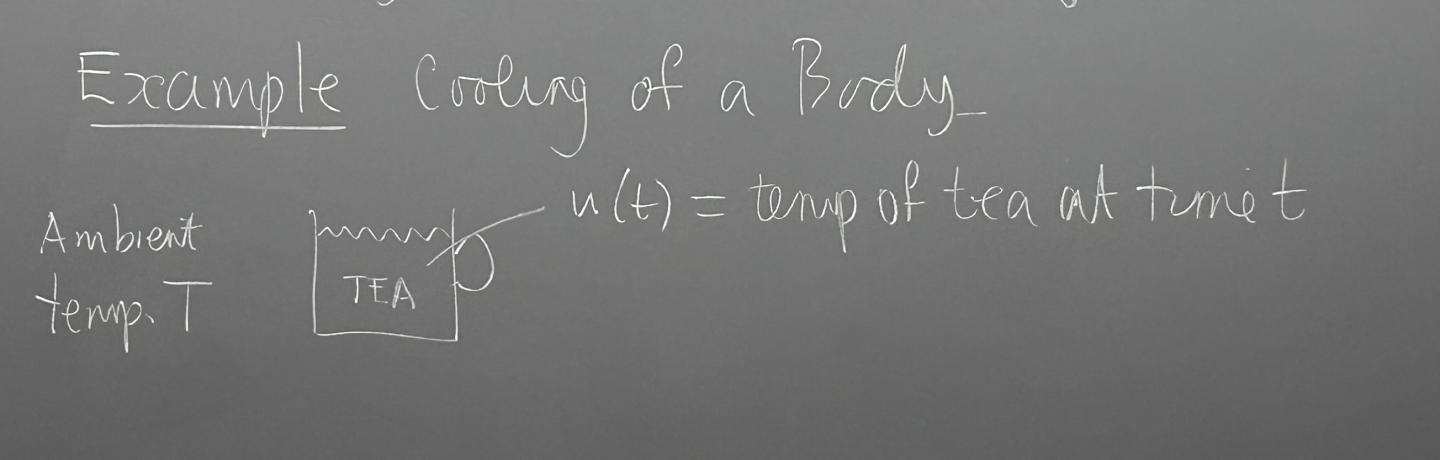
\includegraphics[width=0.6\textwidth]{Figures/lecture1/lec1-1.png}\]
Consider the system at time $t$ and time $t + \delta t$. Hear energy is conserved in this system. The heat energy in the cup at time $t$
 is
 \[m_T c_T u(t)\]
 where $m_T$ is the mass of the tea and $c_T$ is the specific heat capacity of the tea. The heat energy at time $t + \delta t$ is
 \[m_T c_T u(t + \delta t) = m_T c_T u(t) - \{\text{Heat lost to the surroundings}\}\]

\begin{question}
    How much heat is lost?
\end{question}

The amount of heat is lost should be dependent on the difference $u(t) - T$, the surface area of the cup, and should be proporitional to $\delta t$ (provided that it is really small so we can do a local linear approximation). There could also be vapor going out with some convection going out, but we will ignore it for now by Ainsworth's Principle of Maximum Laziness.\\

Hence the amount of heat lost could be modeled as
\[\alpha (u(t) - T) \delta t\]
where $\alpha > 0$ is some constant that measures the ``physical attributes" of the cup.\\

Hence, the heat energy at time $t + \delta t$ can be given as
\[m_T c_T u(t + \delta t) = m_T c_T u(t) - \alpha (u(t) - T) \delta t\]
This equation implies that
\[\frac{ u(t + \delta t) - u(t)}{\delta t} = - \beta (u(t) + T)\]
where $\beta = \frac{\alpha}{m_T c_T} > 0$. Taking the limit as $\delta t \to 0$, we have that
\[u'(t) = - \beta (u(t) - T)\]
Finally, we add an initial condition specifying that $u(t_0) = u_0$.\\

Solving the ODE using standard techniques of calculus, we obtained that
\[u(t) = T + (u_0 - T) e^{-\beta t}, t \geq 0\]

Observe that as $t \to \infty$, we have that
\[u(t) \to T\]

This question is an example of a linear, first order, initial value problem. This is called \textbf{Newton's Law of Cooling}.
 \end{example}

 \begin{example}
     What if we replace the cup of tea with the planetary phenonmenon ``black body"?
     \[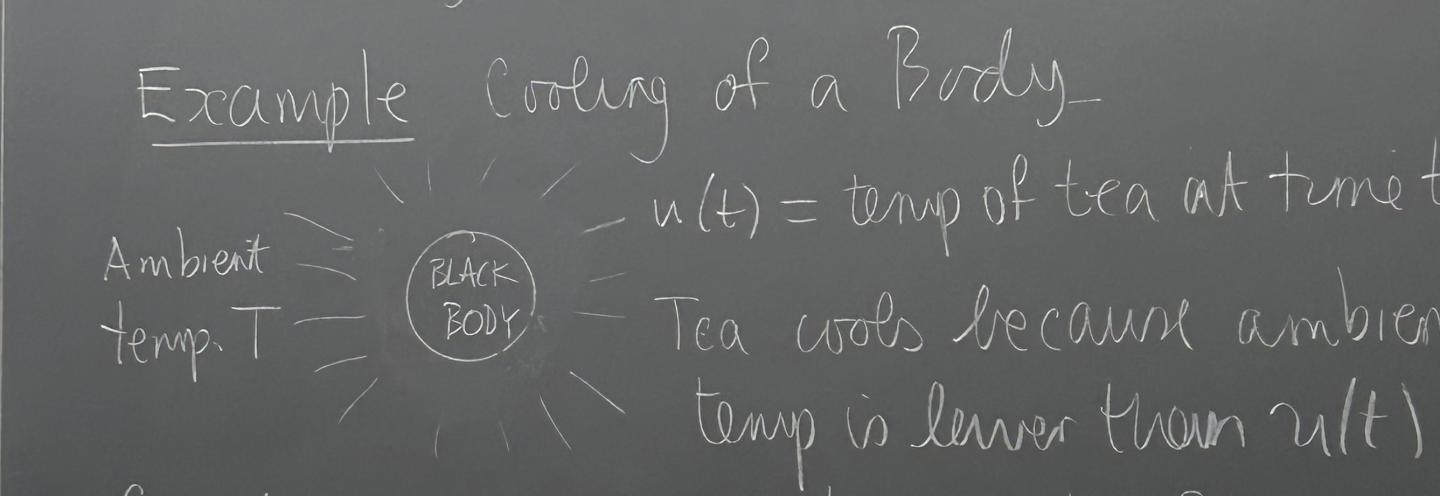
\includegraphics[width=0.6\textwidth]{Figures/lecture1/lec1-2.png}\]
     \textbf{Stefan's Law of Black Body Radiation} says that the heat energy lost should be proportional to $(u(t) - T)^4$ instead of $(u(t) - T)$ and we have
     \[\alpha_1 (u(t) - T) + \alpha_4 (u(t) - T)^4\]
     for $\alpha_1, \alpha_4 \geq 0$.\\

     This leads to an initial valued problem:
     \[u'(t) = - \beta_1 (u(t) - T) - \beta_4 (u(t) - T)^4, u(t_0) = u_0\]
     The solution of this can be done in analytic form, but it is not as easy as the previous example.
     \begin{question}
         How do we proceed from here? It depends on who you ask.
     \end{question}
     \begin{itemize}
         \item \textbf{Dynamical system approach: }In this case, we look for an equilibrium and cosnider the RHS
         \[f(u) = - \beta_1 (u - T) - \beta_4 (u - T)^4\]
         An equilibrium (critical point) is here if and only if $f(u) = 0$.
         
         For example $u = T$ is an example of a equilibrium. $\beta_1 + \beta_4 (u - T)^3 = 0$ is another solutions, which is true if and only if $u = T - (\frac{\beta_1}{\beta_4})^{1/3} < T$. These are the only two equilibriums of the system. The graph looks somewhat like:
       \[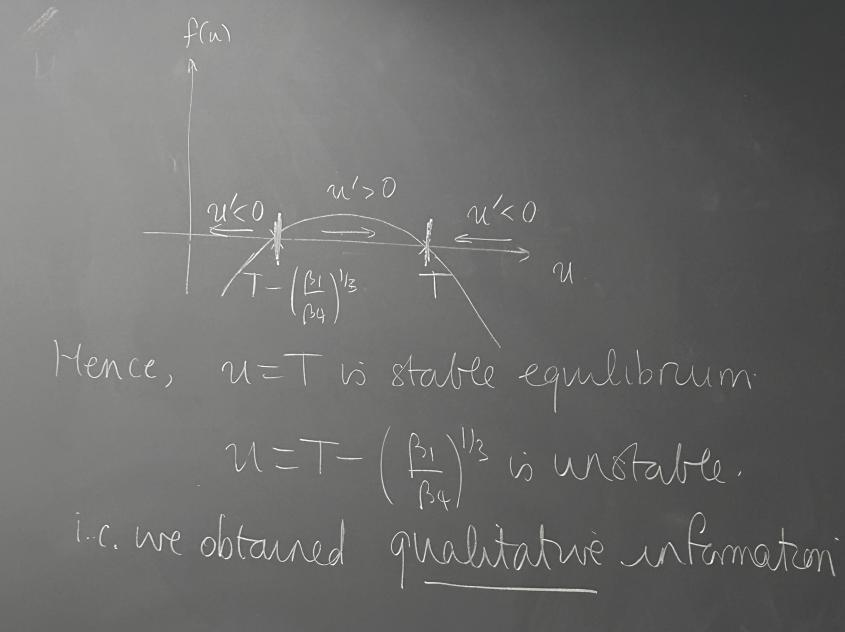
\includegraphics[width=0.6\textwidth]{Figures/lecture1/lec1-3.png}\]
        Hence, $u = T$ is a stable equilibrium and $u = T - (\frac{\beta_1}{\beta_4})^{1/3}$ is an unstable equilibrium. We have obtained \textbf{qualitative information} about the system. However, sometimes we need \textbf{quantitative information} about a system, ie. we want a sufficiently accurate approximatin of this solution.
        
        The physics is also a little dodgy for $t < T - (\frac{\beta_1}{\beta_4})^{1/3}$ since the model implies temperature would run off the negative infinity here.
        \item \textbf{Numerical PDE/ODE approach: } This is how we will get quantitative information. Even then, the type of numerics you want to do could depend on what you are trying to do. For example, if your numerical method does not perserve energy, then to physics this is unacceptable. So you might want to sacrifice accuracy to perserve energy. That's why there are a lot of studies around this topic.

        Numerical PDE/ODE isn't just asking a computer to output some answers. There's a methodology in selecting the right tools and tackling the right questions.
     \end{itemize}
 \end{example}

Let's do another example
\begin{example}[Population Growth]
    Let $N(t)$ be the population at time $t$ and we want to look at how $N(t)$ grows as $t$ changes. The simple method is to model
    \[N(t + \delta t) = N(t) + \delta t [\alpha_B N(t) -  \alpha_D N(t)]\]
    where $\alpha_B \geq 0$ indicates the birth rate and $\alpha_D \geq 0$ indicates the death rate. We have again that
    \[\frac{N(t + \delta t) - N(t)}{\delta t} = (\alpha_B - \alpha_D) N(t)\]
    When we take the limit, we have that
    \[N'(t) = (\alpha_B - \alpha_D) N(t), N(0) = N_0\]
    The behavior as $t \to \infty$ depends on the sign of $\alpha_B - \alpha_D$ as when when solve the equation, we get
    \[N(t) = N_0 e^{(\alpha_B - \alpha_D) t}\]
    Notice that
    \[\lim_{t \to \infty} N(t) = \begin{cases}
    \infty, \alpha_B > \alpha_D\\
    0, \alpha_B < \alpha_D\\
    N_0, \alpha_B = \alpha_D
    \end{cases}\]
This behavior does not make sense in real life, and our model does not account for (finite resources, diseases, etc.)\\

Let $\alpha = \alpha_B - \alpha_D$, let's instead model this as the \textbf{logistics equation}
\[N(t + \delta t) = N(t) + \delta t \alpha N(t) - \delta t \beta N(t)^2 \]
where $\beta$ accounts for resource management and we make the reasonable assumption that resource management squares as population grows. It also tries to take account of diseases, etc. Hence we have that
\[N'(t) = \alpha N(t) - \beta N(t)^2\]

This could be solved analytically, but it is somewhat complicated.

Let's pretend again that we are dynamical systems students, then let
\[f(N) = \alpha N - \beta N^2\]
Then we have that $f(N) = 0$ if and only if $N = 0$ or $N = \frac{\alpha}{\beta} > 0$, and the graph is
\[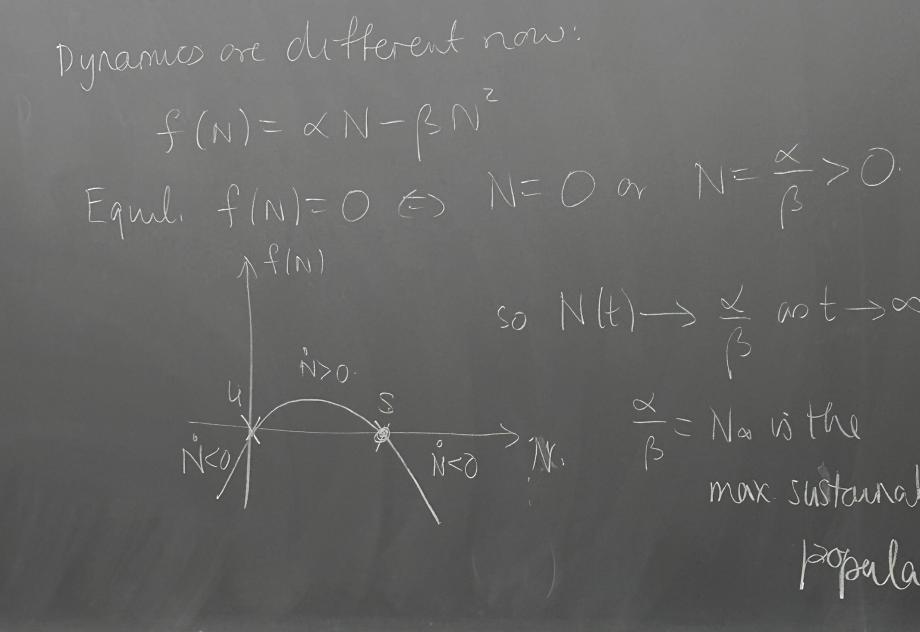
\includegraphics[width=0.6\textwidth]{Figures/lecture1/lec1-4.png}\]
Hence we expect $N(t)$ to tend towards the equilibrium at $\alpha/\beta$. We call $N_\infty = \frac{\alpha}{\beta}$ as the maximum sustainable population.\\

Let's also look at \textbf{spatial effects}, suppose we have an island $\Omega$ where the population is on the island:
\[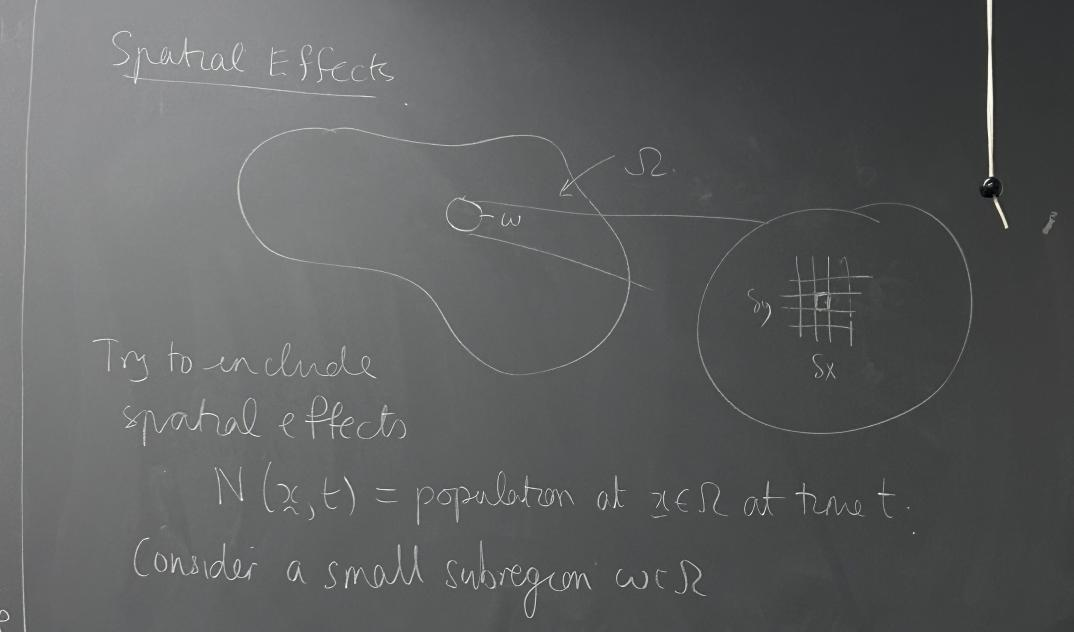
\includegraphics[width=0.6\textwidth]{Figures/lecture1/lec1-5.png}\]
We want $N(x, t)$ to be the population at $x \in \Omega$ and time $t$. Consider a small subregion $\omega \subset \Omega$, and let's let $N_w(t)$ be the population in $\omega$ at time $t$, note that
\[N_w(t) = \int_{w} N(x, t) dx\]
By the principle of conservation of people, we need to take account of the birth and death rate and the immigration rate on the boundary:
\[N_w(t + \delta t) = N_w(t) + \delta t \int_w dx \left(\alpha N(x, t) - \beta N(x, t)^2 \right) - \{\text{immigration at $\partial \omega$ during $(t, t + \delta t)$}\} \]
Let's call a small arc of the boundary as $\delta s$, we make the assumption that people go from more dense place to less dense places.\\

Let's define a flux $\sigma(x, t)$ which is proportional to the spatial gradient $-\nabla N(x, t)$ (the minus sign is here since we are going from more dense places to less dense places). So we write our \textbf{constructive equation}
\[\sigma(x, t) = - \gamma \nabla N, \gamma > 0\]

Hence, the outflow across $\delta s << 1$ should be $\delta s \sigma(x, t) \cdot n$, where $n$ is the unit outward normal vector.
\[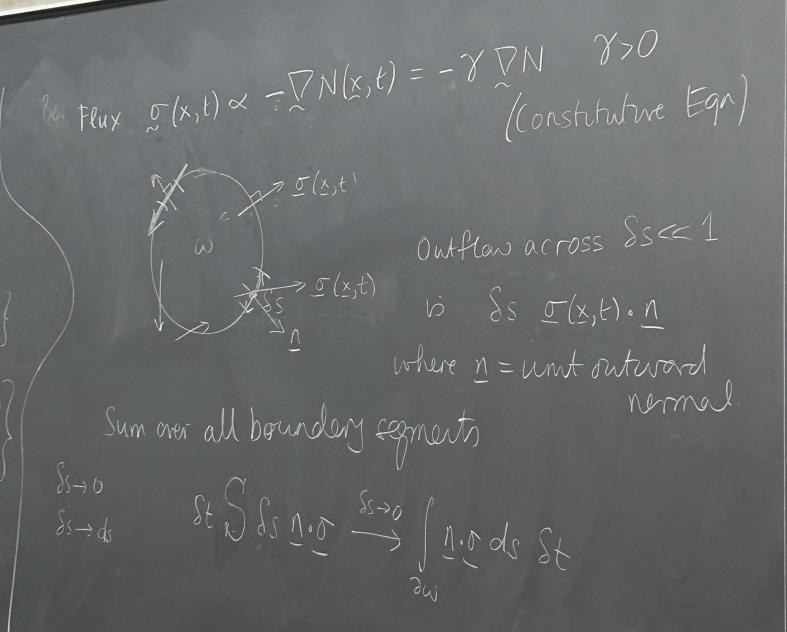
\includegraphics[width=0.6\textwidth]{Figures/lecture1/lec1-6.png}\]
When we sum over all the boundary segments, the immigration effect is 
\[\lim_{\delta s \to 0} \delta t \sum \delta s n \cdot \sigma = \delta t \int_{\partial w} n \cdot \sigma ds \]
Hence, we have that
\begin{align*}
    \int_\omega N(x, t + \delta t) dx &= \int_w N(x, t) dx + \delta t \int_w (\alpha N - \beta N^2) dx - \delta t \int_{\partial w} n \cdot \sigma ds\\
    \iff \int_w \frac{N(x, t + \delta t) - N(x, t)}{\delta t} dx &= \int_w (\alpha N - \beta N^2) dx - \int_w dw \sigma dx \tag*{Divergence Theorem}
\end{align*}
If we take the limit as $\delta t \to 0$ and substitute for $\sigma$, we have that
\[\int_w \frac{\partial N}{\partial t} dx = \int_w (\alpha N - \beta N^2 + \gamma \Delta N) dx\]
for all subregion $w \subset \Omega$. Let ``$w \to 0$" (let the region go smaller and smaller), that is we will divide both side by area of $w$ - $|w|$, and we take $|w| \to 0$:
\[\frac{1}{|w|} \int_w \frac{\partial N}{\partial t} dx = \frac{1}{|w|}  \int_w (\alpha N - \beta N^2 + \gamma \Delta N) dx\]
Assuming $N$ is smooth, taking the limit $|w| \to 0$, we will concentrate at a specific point $x \in w$, gives us
\[\frac{\partial N}{\partial t} = \alpha N - \beta N^2 + \delta \Delta N \text{ in $\Omega$ for $t > 0$}\]
This is called \textbf{Fisher's Equation}. Now we need to supplement this with an initial condition
\[IC: N(x, 0) = N_0(x), x \in \Omega\]
In other words, we should know how many people is at each stop at the beginning. We also need some boundary conditions. The flux at the boundary should be going inward since no one wants to leave the boundary. We want to specify the normal component of the flux should be equal to $0$ on the boundary, hence
\[BC: n \cdot \sigma(x, t) = 0, x \in \partial \Omega\]
Recall that $\frac{\partial N}{\partial n} = n \cdot \nabla N$, hence we have the equivalent condition that
\[\frac{\partial N}{\partial n}(x, t) = 0, x \in \partial \Omega\]
This is an example of a \textbf{reaction-diffusion equation}.
\end{example}

There are no lectures next Wednesday.

\newpage

\section{Lecture 2}

\subsection{More on Fisher's Equation}
Last time, we derived \textbf{Fisher's Equation}  - $N(x, t)$ is the density of a population at $x \in \Omega$ at time $t \geq 0$, and we derived the PDE
\[\frac{\partial N}{\partial t} = \epsilon \Delta N + \mu N (1 - \frac{\lambda}{\mu} N) \text{ in $\Omega$, $t > 0$}\]
subject to the constraint that $N(x, 0) = N_0(x)$ for all $x \in \Omega$, and that
\[\frac{\partial N}{\partial \eta} = 0 \text{ on $\partial \Omega$, $t > 0$}\]
where we derive against the normal component $\eta$ (this is to reflect that the population's normal component with respect to the boundary should be 0 - they shouldn't leave the boundary). This is an interesting \textbf{time dependent PDE}.\\

The term $\epsilon \Delta n$ is thought of as a ``mixing term" in space.

\begin{question}
    How would we solve \textbf{Fisher's equation}? There's no hope of finding an analytic solution to this, so we really want to approximate this using some numerical schemes.
\end{question}

Consider the special case where $\Omega \subset \Rbb$ (ie. we have a 1D domain), we might as well just assume that $\Omega$ is connected as a single interval which we will rescale to $\Omega = (-\pi, \pi)$. We might want to try attacking this using Fourier analysis. Hence, we seek a solution in the form 
\[N(x, t) = \sum_{k = 0}^\infty u_k(t) \cos(kx) \quad (\dagger)\]
We claim this automatically satisfies 
\[\frac{\partial N}{\partial \eta}|_{x = \pm \pi} = 0\]
(In this case we are just taking the derivative in the $+x$ or $-x$ direction), so
\[\frac{\partial}{\partial \eta}|_{x = +\pi} = +\frac{\partial}{\partial x}|_{x = +\pi}\]
\[\frac{\partial}{\partial \eta}|_{x = -\pi} = -\frac{\partial}{\partial x}|_{x = -\pi}\]

We observe that the Fourier coefficients $\{u_k\}_{k = 0}^\infty$ are time dependent (to be determined).
\begin{question}
    How are we gonna find the Fourier coefficients?
\end{question}

We can try to plug this back (substitute the ``Ansatz") into Fisher's equation and compare the Fourier coefficients on both sides. Let's consider the linear parts (in N):
\[\frac{\partial N}{\partial t} - \epsilon \Delta N - \mu N\]
The $m$-th Fourier coefficients of the equation above would be
\begin{align*}
    \frac{d u_m}{dt} + \epsilon m^2 u_m - \mu u_m  
\end{align*}
If we don't have the non-linear term, this is just an ODE in time we could solve readily, but we have a more complicated non-linear part $- \lambda N(x, t)^2$, with $m$-th Fourier coefficient as
\begin{align*}
    \frac{-\lambda}{2\pi} \int_{-\pi}^{\pi} N(x, t)^2 \cos(mx) dx
\end{align*}
Let's write this term as a function $F_m$ and is a function of $t, u_0, u_1, ...$. 

\begin{question}
Putting everything together, on the $m$-th Fourier coefficient, we have that
\[\frac{d u_m}{dt} = - \epsilon m^2 u_m + \mu u_m - F_m(t, u_0, u_1, u_2, ...)\]
where $u_m(0)$ is the $m$-th Fourier coefficient of $N_0(x)$. What's the problem?
\end{question}

Well, we ended up with
\begin{itemize}
    \item An infinite system of ODEs, but we could just try to truncate and approximate using a finite number ($p$) of terms, ie.
    \[N(x, t) \approx \sum_{k = 0}^p u_k(t) \cos(kx)\]
    In practice, we choose $p \sim 100, 1000, ...$
    \item We have a large system of ODEs that is 
    \begin{itemize}
        \item (a) coupled due to a non-linear term $N^2(x,t)$.
        \item (b) the system itself is non-linear.
    \end{itemize}
    \item Needs to be integrated / solved numerically.
    \item Is it even obvious that a solution exists for this equation? If it exists, is the solution unique? Numerical analysis algorithms get a lot harder when solutions don't exist or when solutions are not unique.
\end{itemize}

The last bullet point is what we will investigate first.

\subsection{Existence, Uniqueness, and Well-Posedness of IVP}
Consider a simple scalar initial valued problem
\[\frac{du}{dt} = f(t, u), t > t_0\]
subject to $u(t_0) = u_0$.

\begin{question}
    Does it always have a solution? Is it unique?
\end{question}

Without any assumptions on $f$, there's not much we can say.
\begin{example}[Exists but not unique]
    Let $f(t, u) = 3 u^{2/3}$ and $t_0 = u_0 = 0$ and let's try to solve
    \[u' = 3 u^{2/3}, u(0) = 0\]
    Let $c > 0$ be any constant and define
    \[u_c(t) = \begin{cases}
        (t - c)^3, t \geq 0\\
        0, c > t \geq 0
    \end{cases}\]
    It's easy to check that $u_c(t)$ satisfies the ODE. However, the solution here is clearly not unique.
\end{example}

\begin{example}
    Let $p = 0$ (number of ODEs) in Fisher's equation and write it as the equation $\frac{du}{dt} = \mu u - \lambda u^2$ is the logistic equation. This is because we can look at 
    \[\frac{du_0}{dt} = \mu u_0 - \lambda \frac{1}{2\pi} \int_{-\pi}^{\pi} N(x, t)^2 dx = \mu u_0 - \lambda u^2\]
    Let's might as well get rid of $\mu$ and take $\lambda = 1$, so we have that
    \[f(t, u) = - u^2, t_0 = u_0 = -1\]
    This is reminiscent of a simplified Fisher/Logistic Equations. Let's try to solve
    \[\frac{du}{dt} =  - u^2\]
    Here we have that
    \begin{align*}
        \frac{du}{dt} =  - u^2 &\iff \int -\frac{du}{u^2} = \int dt\\
        &\iff \frac{1}{u} = t + C
    \end{align*}
    So $C = 0$ satisfies, so we have solution $u(t) = \frac{1}{t} + C$. In this case a solution exists, but it is only defined up to $t = 0$, it could never get to positive time!
\end{example}

\begin{question}
    What kind of assumption should we place on $f$ to get existence and uniqueness?
\end{question}

\begin{definition}[Lipschitz Continuous]
    Let $S \subseteq \Rbb$ and $F: S \to \Rbb$, then $F$ is Lipschitz on $S$ if there exists some constant $L$ such that
    \[|F(u) - F(v)| \leq L |u - v|, \forall u, v \in S\]
\end{definition}

\begin{example}
    Here are some examples
    \begin{itemize}
        \item Let $F(x) = 3x^{2/3}$ is not Lipschitz continuous on any interval containing $0$. In this case
        \[\lim_{x \to 0} \frac{|x^{3/2} - 0|}{|x - 0|} = \infty\]
        \item Let $F(x) = -x^2$ is not Lipschitz on $\Rbb$ since
        \[\frac{|u^2 - v^2|}{|u - v|} = |u + v| \text{blows up on $u$ and/or $v \to \pm \infty$} \]
    \end{itemize}
\end{example}

\begin{remark}
   When the instructor was in his undergraduate days, he was in a math society. Once upon a time, they invited Robin Wilson (who is a mathematician and the son of a British politician) to come give a math talk. Robin Wilson really likes collecting mathematical stamps of some sorts. In the talk, Robin Wilson gave a talk about stamps.\\

    One of the professors in the audience asked:
    \begin{itemize}
        \item "You have shown us all sorts of mathematical stamps, but do you know any stamps that have nothing to do with mathematics?"
    \end{itemize}
   Robin Wilson, being a precise mathematician, thought about this question for a while and answered:
   \begin{itemize}
       \item ``No, there are no stamps that have nothing to do with mathematics".
   \end{itemize}
\end{remark}

\begin{proposition}
    Suppose $S$ is closed and bounded and $F: S \to \Rbb$ is continuously differentiable, then $F$ is Lipschitz on $S$.
\end{proposition}

\begin{proof}
    We have that
    \begin{align*}
        |F(u) - F(v)| &= |\int_{v}^u F'(s) ds|\\
        &\leq |u - v| \max_{x \in S} |F'(x)|\\
        &= |u - v| L \tag*{Since $S$ is compact}
    \end{align*}
\end{proof}

\begin{theorem}[Picard's Theorem]
    Let $R = [t_0 - h, t_0 + h] \times [u_0 - k, u_0 + k]$ and suppose $f: R \to \Rbb$ is continuous with 
    \begin{enumerate}
        \item $|f(t, u)| \leq M_0$ for $(t, u) \in \Rbb$.
        \item Lipschitz with respect to the second variable, ie. for a fixed $t$
        \[|f(t, u) - f(t, v)| \leq M_1 |u - v|\]
        for $(t, u), (t, v) \in R$.
    \end{enumerate}
    If $M_0 h \leq k$ and $M_1 h < 1$ (so $h$ has to be sufficiently small), then the problem 
    \[\frac{du}{dt} = f(t, u), u(t_0) = u_0\]
    has a unique solution that is continuously differentiable $\varphi$ defined on $I = (t_0 - h, t_0 + h)$ satisfying
    \begin{itemize}
        \item  $\varphi(t_0) = u_0$.
        \item $\varphi(t) \in [u_0 - k, u_0 + k]$ for all $t \in I$.
        \item $\frac{d\varphi}{dt} = f(t, \varphi(t))$ for all $t \in I$.
    \end{itemize}
\end{theorem}

\begin{remark}
    The larger the $k$ is, the less you can say about the certainity of $\varphi(t)$. The larger $h$ is, the better we could say about the domain $I$.
\[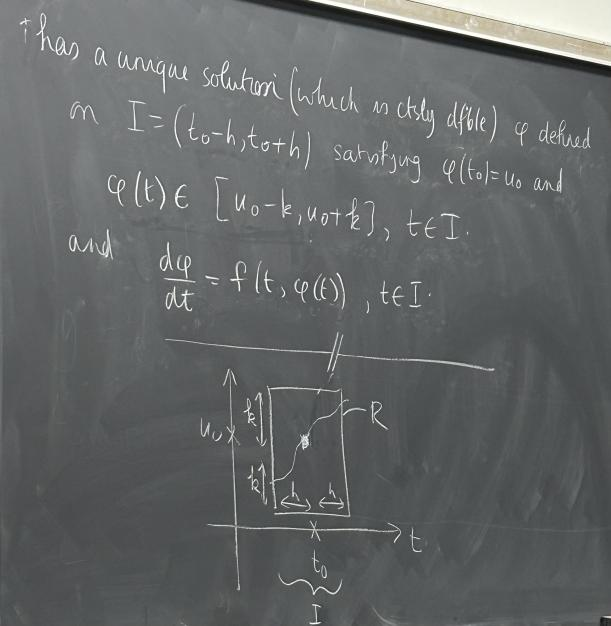
\includegraphics[width=0.6\textwidth]{Figures/lecture2/lec2-1.png}\]
    We would like to have $k$ small and $h$ large.
\end{remark}

\begin{remark}
    In this class, ``continuously differentiable" means the function is continuous, is differentiable, and the derivative is continuous.
\end{remark}

We need a couple of tools before proving Picard's Theorem:
\begin{enumerate}
    \item Let $C(I)$ be the space of bounded continuous functions on $I$ equipped with the $\ell^\infty$-norm
    \[||f|| = \sup_{t \in I} |f(t)|\]
    It has the following property:
    \begin{itemize}
        \item If there's a Cauchy sequenece $\{f_k\} \in C(I)$ such that $||f_k \to f_\ell|| \to 0$ as $k, \ell \to 0$, then there exists a limit $f \in C(I)$ such that
        \[\lim_{t \to \infty} ||f - f_t|| = 0\]
        (This is just saying that $\ell^\infty$ is complete). This is not too difficulty to prove, but we will omit it in class.
    \end{itemize}
    \item We need the following lemma
    \begin{lemma}
        Let $a < b$ and define the subset $E \subset C(I)$ by
        \[E = \{ f \in C(I) : a \leq f(t) \leq b, t \in I \}\]
        Suppose we have a sequence of functions $\{f_k\}$ in $E$ that converges to $f$, then $f \in E$.
    \end{lemma}

    \begin{remark}
        This just means that $E$ is a closed subspace of $C(I)$. Closed subspace of a complete metric space is a complete metric space.
    \end{remark}

    \begin{proof}
        Let $k \in \Nbb$, so $a \leq f_k(t) \leq b$ for all $t \in I$. For any $\epsilon > 0$, there exists $N$ such that
        \[|| f - f_n || < \epsilon \text{ for all $n > N$}\]
        \[\iff -\epsilon < f(t) - f_n(t) < \epsilon \text{ for all $n > N$}\]
        \[\iff a - \epsilon \leq f_n(t) - \epsilon < f(t) < f_n(t) + \epsilon \leq b + \epsilon\]
        This implies that $a + \epsilon < f(t) < b + \epsilon$ for all $t \in I$. Let $\epsilon \to 0$, we get that $f \in E$.
    \end{proof}
\end{enumerate}

\begin{proof}[Proof of Picard's Theorem]
    We seek a function $\varphi \in C(I)$, $\varphi(t) \in [u_0 - k, u_0 + k]$ for all $t \in I$, and
    \[\varphi(t) = u_0 + \int_{t_0}^t f(s, \varphi(s)) ds, \forall t \in I\]
    This is equivalent to saying $\frac{d\varphi}{dt} = f(t, \varphi(t))$ with initial conditions $\varphi(t_0) = u_0$ using the Fundamental Theorem of Calculus. In other words, we want to show $\varphi \in E$ with $a = u_0 - k$ and $b = u_0 + k$.\\

    Now, given an arbitrary function $\zeta \in E$, we define a new function
    \[\psi(t) = u_0 + \int_{t_0}^t f(s, \zeta(s)) ds, \forall t \in I\quad (\star)\]
    Observe that $\psi \in C(I)$. Clearly it is continuous, for boundedness, note that $(s, \zeta(s)) \in R$, we have that
    \[|\psi(t) - u_0| \leq |t - t_0| \sup_{s \in I} |f(s, \zeta(s))| \leq |t - t_0| M_0 \leq h M_0 \leq k\]
    where the last inequality comes from assumption of the theorem. Hence, $\psi(t) \in [u_0 - k, u_0 + k]$ for all $t \in I$. We conclude that $\psi \in E$.\\

    Consequently, $(\star)$ defines a mapping $T: E \to E$ by the rule $\psi = T(\zeta)$. Let $\zeta_1, \zeta_2 \in E$ and $\psi_1 = T(\zeta_1), \psi_2 = T(\zeta_2)$. Then
    \begin{align*}
        |\psi_1(t) - \psi_2(t)| &= |\int_{t_0}^t \{f(s, \zeta_1(s)) - f(s, \zeta_2(s))\} ds|\\
        &\leq |\int_{t_0}^t M_1 |\zeta_1(s) - \zeta_2(s)| | \tag*{Lipschitz in second variables}\\
        &\leq M_1 \sup_{s \in I} |\zeta_1(s) - \zeta_2(s)| |t - t_0|\\
        &= M_1 h ||\zeta_1 - \zeta_2||,\quad \forall t \in I
    \end{align*}
    Hence we have that
    \[||\psi_1 - \psi_2|| \leq M_1 h ||\zeta_1 - \zeta_2|| \quad (*)\]
    Now since $M_1 h < 1$ by assumption, the rest follows from \textbf{Banach's fixed point theorem}, but not everyone in the class knows this result! So we will proceed....\\

    Define a sequence $\{\varphi_n\}_{n=0}^\infty$ by the rule
    \[\varphi_0(t) = u_0, t \in I\]
    \[\varphi_{n+1} = T(\varphi_n), n = 0, 1, ....\]
    Hence, since $\varphi_0 \in E$ and since $T: E \to E$, we have a whole sequence in $E$. We will check this is a Cauchy sequence, let $m > n$, by Triangle's inequality and ``bootstrapping" this inequality, we have that
    \begin{align*}
        ||\varphi_m - \varphi_n|| &\leq ||\varphi_{m} - \varphi_{m-1}|| + ... + ||\varphi_{n+1} - \varphi_n||\\
        &\leq \sum_{\ell = 0}^\infty ||\varphi_{n + \ell + 1} - \varphi_{n + \ell}|| \\
        &\leq \sum_{\ell = 0}^\infty (M_1 h)^{n+\ell} ||\varphi_1 - \varphi_0||  \tag*{Using $(*)$}\\
        &= (M_1 h)^n  ||\varphi_1 - \varphi_0|| \sum_{\ell = 0}^\infty (M_1 h)^{\ell}\\
        &= (M_1 h)^n ||\varphi - \varphi_0|| \frac{1}{1 - M_1 h}
    \end{align*}
    Therefore, $||\varphi_m - \varphi_n|| \to 0$ as $n, m \to \infty$. This is a Cauchy seuqnece in $E$, so our lemma tells us that the limit $\varphi$ of this sequence is in $E$.\\

    Now, $||\varphi - T(\varphi)|| = ||\varphi - \varphi_{n+1} + \varphi_{n+1} - T(\varphi)|| \leq ||\varphi - \varphi_{n+1}|| + ||T(\varphi_n) - T(\varphi)|| \leq ||\varphi - \varphi_{n+1}|| + (M_1 h)||\varphi_n - \varphi||$ which tends to $0$ as $n \to \infty$, hence we verify that $\varphi$ is a fixed point of the integral equation earlier.\\

    For uniqueness, suppose there's another $\Tilde{\varphi} \in E$ such that $\Tilde{\varphi} = T(\Tilde{\varphi})$ but $\Tilde{\varphi} \neq \varphi$, then consider
    \begin{align*}
        ||\varphi - \Tilde{\varphi}|| &= ||T(\varphi) - T(\Tilde{\varphi})||\\
        &\leq M_1 h ||\varphi - \Tilde{\varphi}||\\
        &< ||\varphi - \Tilde{\varphi}|| \tag*{$M_1 h < 1$}
    \end{align*}
    which is a contradiction. Hence we conclude that $\varphi$ is unique.
\end{proof}

\begin{remark}
    This is a constructive argument to make $\varphi$. However, it is not so popular because the map $T$ tends to be difficult to compute.
\end{remark}

\newpage
\section{Lecture 3}

\subsection{More on Picard's Theorem}
Recall - last lecture, we proved Picard's Theorem:
\begin{theorem}[Picard's Theorem]
    Let $R = [t_0 - h, t_0 + h] \times [u_0 - k, u_0 + k]$ and suppose $f: R \to \Rbb$ is continuous with 
    \begin{enumerate}
        \item $|f(t, u)| \leq M_0$ for $(t, u) \in \Rbb$.
        \item Lipschitz with respect to the second variable, ie. for a fixed $t$
        \[|f(t, u) - f(t, v)| \leq M_1 |u - v|\]
        for $(t, u), (t, v) \in R$.
    \end{enumerate}
    If $M_0 h \leq k$ and $M_1 h < 1$ (so $h$ has to be sufficiently small), then the problem 
    \[\frac{du}{dt} = f(t, u), u(t_0) = u_0\]
    has a unique solution that is continuously differentiable $\varphi$ defined on $I = (t_0 - h, t_0 + h)$ (note that this is open) satisfying
    \begin{itemize}
        \item  $\varphi(t_0) = u_0$.
        \item $\varphi(t) \in [u_0 - k, u_0 + k]$ for all $t \in I$.
        \item $\frac{d\varphi}{dt} = f(t, \varphi(t))$ for all $t \in I$.
    \end{itemize}
\end{theorem}

What this theorem is really saying is that, given the initial condition $(t_0, u_0)$, there's some rectangle around the initial condition $(t_0, u_0)$: 
\[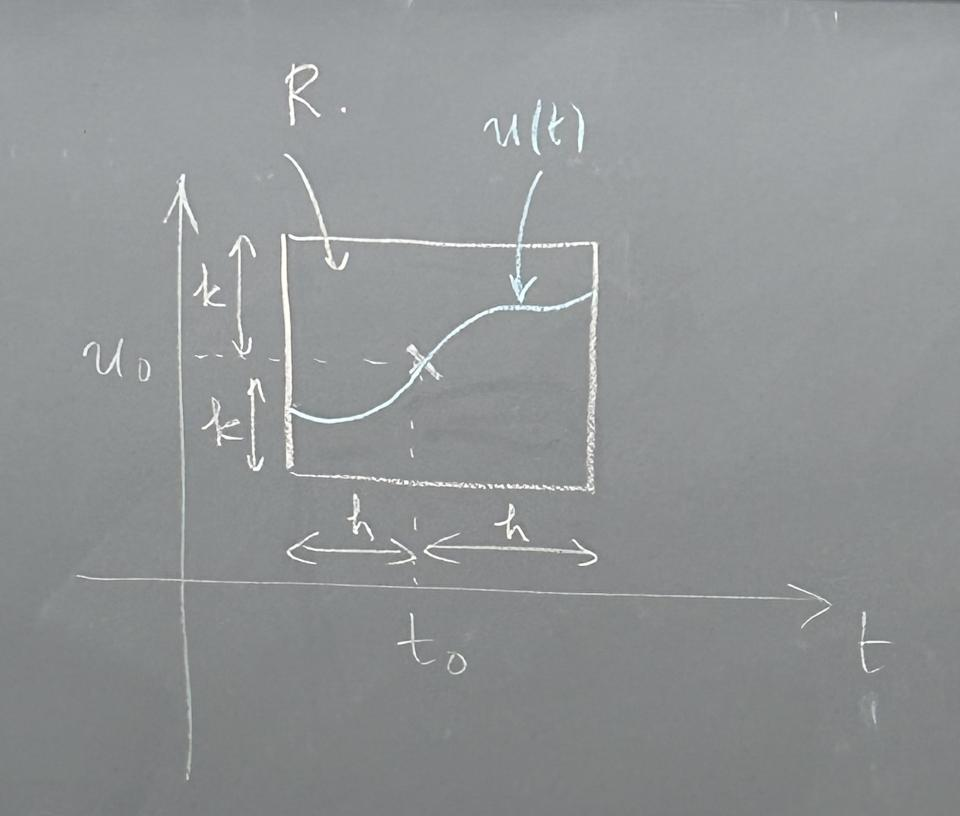
\includegraphics[width=0.6\textwidth]{Figures/lecture3/lec3-1}\]
such that $h$ has to be sufficiently small (recall $M_0 h \leq k$ and $M_1 h \leq k$), $t$ has to be sufficiently large, and thus $u(t)$ exists and is unique.

\begin{example}
    We will again consider a simple problem where $f(t, u) = -u^2$ and $u_0 = t_0 = 1$. We saw before that a solution exists only for $t > 0$. In other words, the global solution $u(t) = \frac{1}{t}$ is only defined to $t > 0$.\\

    Now, let's pretend the global solution is unknown and use Picard's theorem to give a local solution. Let's choose $r = [1 - h, 1 + h] \times [1 - k, 1 + k]$ where $h$ and $k$ are to be determined. Now, we check that
    \[|f(t, u)| = |-u^2| \leq (1 + k)^2 = M_0\]
    Also, we need to look at
    \[|f(t, u_1) - f(t, u_2)| = |u_1^2 - u_2^2| = |u_1 - u_2| |u_1 + u_2| \leq |u_1 - u_2| (|u_1| + |u_2|) \leq 2(1 + k) |u_1 - u_2|\]
    Hence we can take $M_1 = 2 (1 + k)$. We require $h$ and $k$ such that
    \[M_0 h \leq k \text{ and } M_1 h < 1\]
    This is equivalent to requiring that
    \[h \leq \frac{k}{(1 + k)^2} \text{ and } h < \frac{1}{2(1 + k)}\]
    We try to choose $h$ as large as possible to make the domain on which solutions exist as large as possible. This is comparing two curves:
\[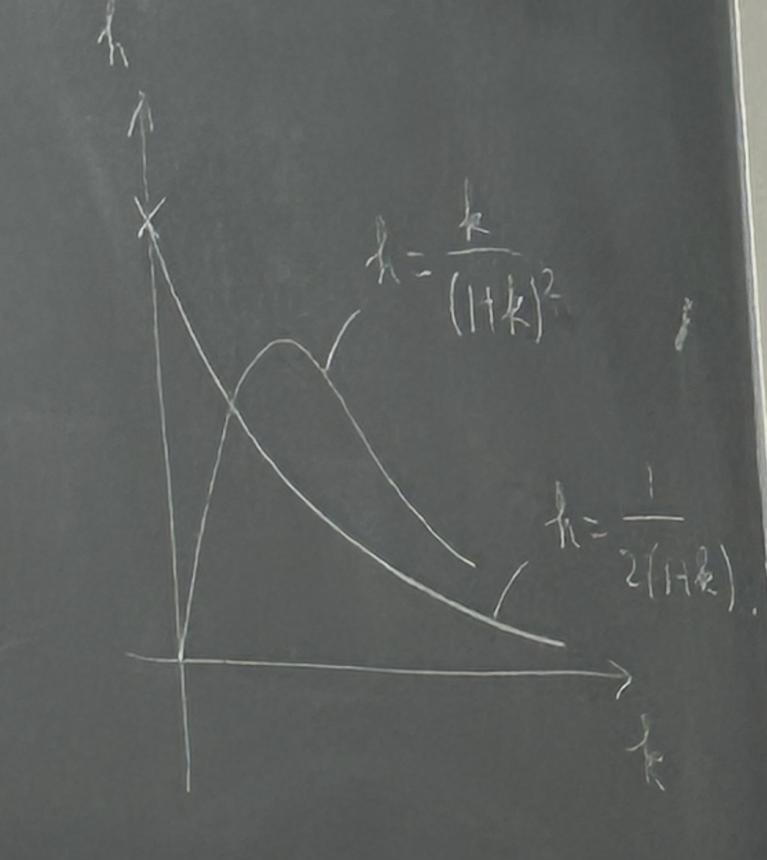
\includegraphics[width=0.4\textwidth]{Figures/lecture3/lec3-2}\]
    The largest value of $h$ is when the two curves intersect, which is at
    \[\frac{k}{(1 + k)^2} = \frac{1}{2(1 + k)} \iff k = 1\]
    Hence, the optimal choice is to take $k = 1$ and $h < 1/4$. Picard's Theorem then tells us that this initial valued problem has a unique solution on $R = [t_0 - h, t_0 + h] \times [u_0 - k, u_0 + k] = [\frac{3}{4}, \frac{5}{4}] \times [0, 2]$. The picture we should keep in mind is
\[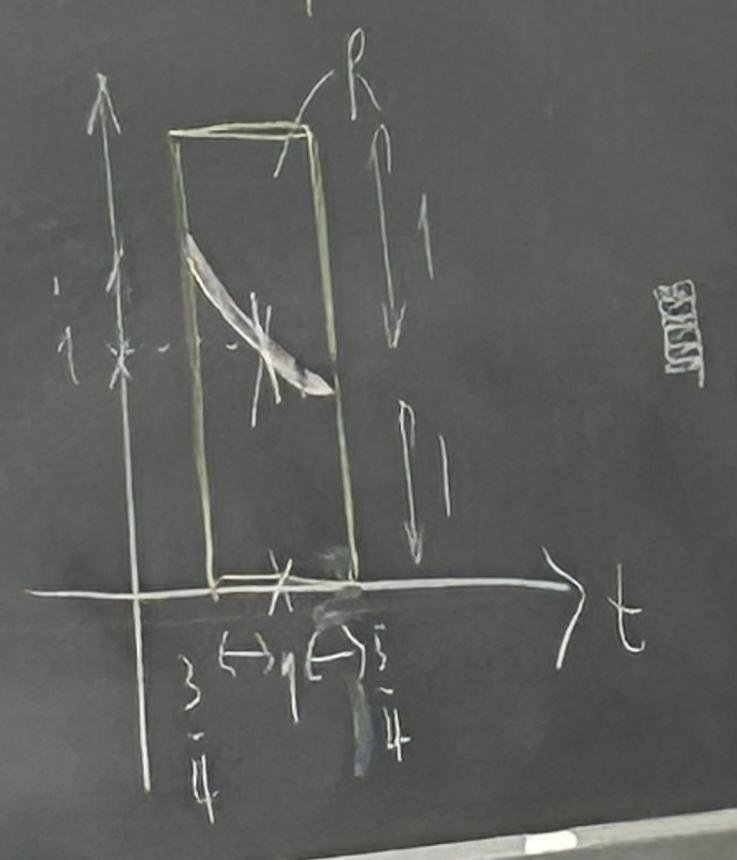
\includegraphics[width=0.4\textwidth]{Figures/lecture3/lec3-3}\]
\end{example}

\begin{question}
    Picard's Theorem told us about existence on $(3/4, 5/4)$, but we know that the solution exists on $(0, \infty)$. This result is not optimal. Can we try to extract some more information out of this? How to ``continue" (note that this is a pun)? 
\end{question}

Why don't we try to look at a point $(t_1, u_1)$ with $t_1 > t_0$, and make a new rectangle. Then we glue the rectangles together if the solutions agree. Then we try to do it for $t_2 > t_1$, etc.
\[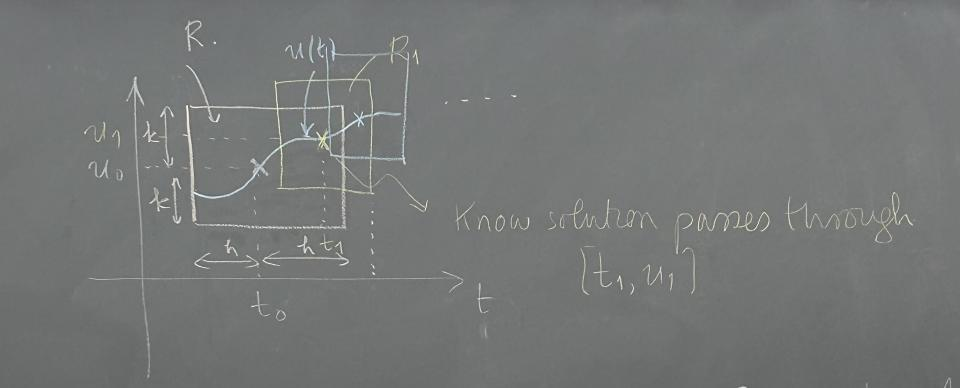
\includegraphics[width=0.8\textwidth]{Figures/lecture3/lec3-4}\]
Observe that the size of $I$ depends on $h$, which in turn only depends on $M_0$, $M_1$, and $k$, but not on the solution $\phi$ we constructed. This means that we can restart / continue the process of a new point $t_1$ such that $u(t_1) = u)1$, and extend to a new rectangle $R_1$.\\

We also notice that the new function $\varphi_1$ agrees with $\varphi$ on the common domain of definition by uniqueness of the solution. There is however one issue with this ``gluing method":
\begin{enumerate}
    \item What if the rectangle keeps shrinking until we eventually can't generate solutions to the entire interval?
\end{enumerate}

\begin{remark}
    If there's no limit on how large $h$ can be (ie. in the set up of the homework last week) in the case where we have a globally Lipschitz condition, we could always find the solution for the entire interval of definition.
\end{remark}

\begin{example}[Example Continued]
    Let's suppose that we start at a new point $t_0$ and $u_0 = \frac{1}{t_0}$, where $t_0$ could be $3/4$ or $5/4$ (from where we left off). Let $R = [t_0 - h, t_0 + h] \times [u_0 - k, u_0 + k]$ where $h$ and $k$ are to be determined again. Then, we have that
    \[|f(t, u)| = |u^2| \leq (u_0 + k)^2 = M_0\]
    \[|f(t, u_1) - f(t, u_2)| \leq |u_1 - u_2| 2(u_0 + k),\quad \text{ hence } M_1 = 2(u_0 + k)\]
    Now we require that $M_0 h \leq k$ and $M_1 h < 1$, which is equivalent to requiring
    \[h \leq \frac{k}{(u_0 + k)^2} \text{ and } h < \frac{1}{2(u_0 + k)}\]
    The optimal choice is when the two curves equal and is when $k = u_0$. Hence $h < \frac{1}{2(u_0 + k)} = \frac{1}{4(u_0)} = \frac{t_0}{4}$. Hence, by Picard's Theorem, the new (extended) interval is 
    \[(t_0 - h, t_0 + h) = (\frac{3 t_0}{4}, \frac{5 t_0}{4})\]
    which agrees with what we had when $t_0 = 1$. If we keep repeating this, we will get the interval after $n$ steps as
    \[(t_0 (\frac{3}{4})^n, t_0 (\frac{5}{4})^n)\]
    Hence, we get the interval $(0, \infty)$ as we take $n \to \infty$.
\end{example}

\begin{remark}
    Picard's theorem extends to systems of first order ODEs for, (ex. in the case of approximating Fisher's equation):
    \[\frac{d\Vec{u}}{dt} = \Vec{f}(t, \Vec{u}), \Vec{u} = (u_0, u_1, ..., u_{N-1}) \]
    where $\Vec{f}: \Rbb \times \Rbb^N \to \Rbb^N$ is bounded and continuous on some hyper-rectangle $R \subseteq \Rbb \times \Rbb^N$ and Lipschitz in all $\Vec{u}$-variables. The proof is almost exactly the same.\\

    Picard's theorem also extends to higher order ODEs:
    \[\frac{d^n u}{dt^n}(t) = f(t, u, \frac{du}{dt}, ..., \frac{d^{N-1} u}{dt^{N-1}}), N > 1\]
    We can change this into a system of first order ODEs as follows - we introduce new variables:
    \[u_0 = u, u_1 \coloneqq \frac{du}{dt}, ..., u_{N-1} \coloneqq \frac{d^{N-1}u}{dt^{N-1}} \]
    Let's set $\Vec{u} = [u_0, u_1, ..., u_{N-1}]$. This then gives us that
    \[\frac{d\Vec{u}}{dt} = [u_0', u_1', ..., u_{N-1}'] = [u_1, u_2, ..., u_{N-1}, \frac{d^N}{dt^N} u] = [u_1, u_2, ..., u_{N-1}, f]\]
    which we just talked about before.
\end{remark}

\subsection{Numerical Quadrature}
We are interested in IVPs of the form
\[\frac{du}{dt} = f(t, u)\]
using an numerical approach. However, even if $f(t, u)$ is independent of $u$, we still have an issue:\\

\begin{question}
Consider the set up
\[\frac{du}{dt}(t) = g(t), t > t_0 \text{ subject to } u(t_0) = u_0\]

We know the exact solution should be
\[u(t) = u_0 + \int_{t_0}^t g(s) ds,\quad t > t_0\]
However, in general this integral might be very difficult to compute analytically! We need to somehow approximate the integral.
\end{question}

Consider a new set up as follows - Suppose we solve a function $u(t)$ from $t = t_0$ to $t = T$,
\[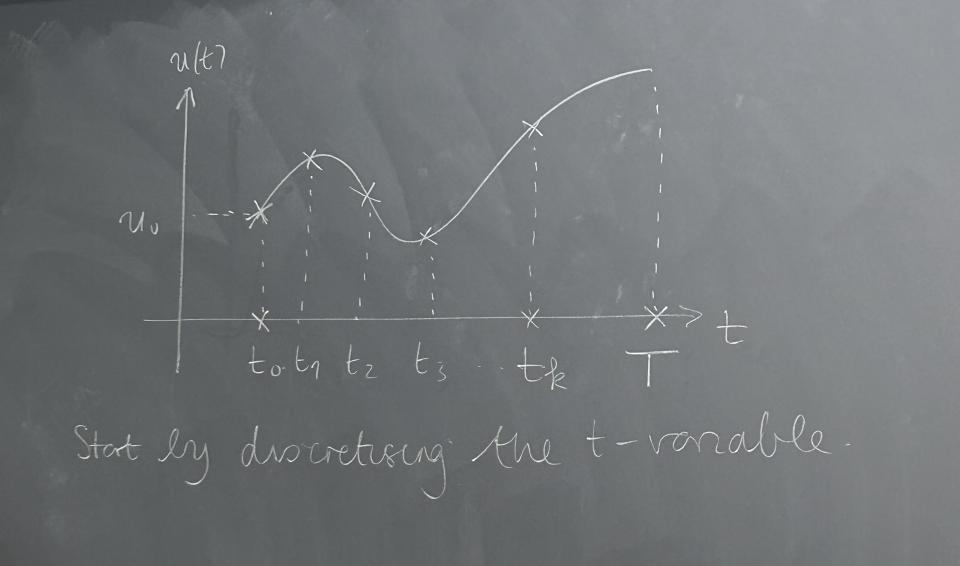
\includegraphics[width=0.5\linewidth]{Figures//lecture3/lec3-5.png}\]
We start by a uniform discretization of the $t$-variables. We define $t_k = t_0 + k h$ where $h = \frac{T - t_0}{n}$ and $n \in \Nbb$. We then try to compute the coordinates $(t_k, u(t_k))_{k = 0}^n$. We know that
\[u(t_1) = u_0 + \int_{t_0}^{t_1} g(s) ds\]
If $h = t_1 - t_0$ is small, then we should be able to approximate the integral ``well". For example, we could use the Trapezoidal rule,
\[\int_0^{h} g(s) ds \approx \frac{h}{2} \{g(0) + g(h)\}\]
This leads to a numerical algorithm:

\begin{tcolorbox}[standard jigsaw,opacityback=0]
\begin{algorithm}[H]
\caption{Trapezoidal Approximations}
\KwData{$u_0$ and $g$}
\KwResult{The tuples approximating $(t_k; u(t_k))_{k = 0}^n$}
1. Choose $n$ and set $h = \frac{T - t_0}{n}$\;
2. For $k = 1, 2, ...$, set $u_k = u_{k-1} + \frac{1}{2} h [g(t_{k-1}) + g(t_k)]$
\end{algorithm}
\end{tcolorbox}

There are however some issues
\begin{enumerate}
    \item How good are the results? We want to estimate $|u(t_k) - u_k|$.
    \item Does the method converge as $h \to 0$. In other words,
    \[\max_{0 \leq k \leq n} |u(t_k) - u_k| \to 0 \text{ as } h \to 0\]
    \item If it does converge, what conditions are on $g$? How fast does this converge? The speed should depend on $g$ and the choice of the quadrature rule.
\end{enumerate}

\begin{question}
    What other kinds of quadrature rule are possible?
\end{question}
\begin{itemize}
    \item Trapezoidal rule: $\int_0^h g(s) ds \approx \frac{h}{2} [g(0) + g(h)]$.
    \item Simpson's rule: $\int_0^h g(s) ds \approx \frac{h}{6} [g(0) + 4 g(\frac{h}{2}) + g(h)]$.
    \item Gauss-Legendre 2-point rule: $\int_0^h g(s) ds \approx \frac{h}{2}\{g(\xi_+) + g(\xi_-)\}$ where $\xi_\pm = \frac{h}{2}(1 \pm \frac{1}{\sqrt{3}})$.
    \item The Midpoint Rule (or Gauss-Legendre 1-point rule): $\int_0^h g(s) ds \approx h g(\frac{h}{2})$.
    \item Left-Hand Endpoint Rule: $\int_0^h g(s) ds \approx h g(0)$.
    \item ... and may others.
\end{itemize}
Any one of these could be used in our algorithm, so how do we know which to choose? There's no clear cut answer because it depends on what we are trying to do. We are interested in the following quantities:
\begin{itemize}
    \item Cost (Number of evaluations of $g$)
    \item Rate of convergence
    \item Accuracy
\end{itemize}

In order to answer these questions, we need rigorous error estimates on the quadrature rules. 
\begin{definition}
Assuming the function $g \in C[0, h]$ (it is continuous on $[0, h]$), let $I(g)$ be any of the quadrature rules, then the error function is defined as
\[g(s) \mapsto E(g) \coloneqq \int_0^h g(s) ds - I(g) \]
This is a linear functional $E$ in $\Hom(C[0, h], \Rbb)$. The point is that $E$ (and also $I$) acts on functions, so to be precise, we can write
\[E[t \mapsto g(t)] = \int_0^h g(s) ds - I[t \mapsto g(t)]\]
This will become important later.
\end{definition}

\begin{remark}
One time in the coffee room, the instructor was talking about Gaussian quadratures with his advisor. Roy Roberts heard and conversation and asked "What is the Gaussian quadrature"? Then the instructor's advisor explained. Roy Robert then asks - what happens when we have a function that is continuous nowhere? The instructor's advisor thought about it and then said "They don't usually come up in practice".
\end{remark}

\begin{example}
    Here are some examples of the error functional.
    \begin{enumerate}
        \item If the rule is the Trapezoidal rule, then
        \[E[t \mapsto g(t)] = \int_0^h g(s) ds - \frac{h}{2} [g(0) + g(h)]\]
        If $g(t) = 1$ is the constant function, then
        \[E[t \mapsto 1] = \int_0^h ds - \frac{h}{2}[1 + 1] = 0\]
        If $g(t) = t$, then
        \[E[t \mapsto t] = \int_0^h s ds - \frac{h}{2}[0 + h] = 0\]
        If $g(t) = t^2$, then
        \[E[t \mapsto t^2] = \int_0^h s^2 ds - \frac{h}{2}[0 + h^2] = -\frac{1}{6} h^3\]
    Since $E$ is a linear functional, we conclude that
    \[E[t \to p(t)] = 0 \quad \forall \text{p that is a polynomial of degree at most $1$.}\]

        \item If the rule is the midpoint rule, then
        \[E[t \mapsto g(t)] = \int_0^h g(s) ds - \frac{h}{2} [g(h/2)]\]
        We will again have that $E[t \mapsto 1] = 0$ and $E[t \mapsto t] = 0$. Now,
        \[E[t \mapsto t^2] = \frac{1}{12} h^{3}\]
        So $E[p] = 0$ for all linear polynomials $p$.

        \item If the rule is the two point Gauss-Legendre rule, then
        \[E[t \mapsto g(t)] = \int_0^h g(s) ds - \frac{h}{2} \{g(\xi_+) - g(\xi_-)\}\]
        where $\xi_{\pm} = \frac{h}{2} (1 \pm \frac{1}{\sqrt{3}})$. In this case we still have $E[t \mapsto 1] = 0$ and $E[t \mapsto t] = 0$. Furthermore, $E[t \mapsto t^2] = 0$ and in fact even $E[t \mapsto t^3] = 0$. However, $E[t \mapsto t^4] \neq 0$. In fact, we have that $E[p] \equiv 0$ for all polynomials $p$ with degree less than or equal to $3$. In fact, this the maximal precision, no 2-point rule can eliminate more polynomials than the two point Gauss-Legendre rule.\\

        In general, given $E[t \mapsto g(t)]$, we note that
        \[E[t \mapsto g(t)] = E[t \mapsto g(t) - p_3(t)], \forall p_3 \in \Pbb_3\]
        (here $\Pbb_n$ means all polynomials with degree less than or equal to $n$). Hence, if we could find a good approximation of $g(t)$ using cubics, we could get a good error!
    \end{enumerate}
\end{example}

\begin{conjecture}
    If $E[p] \equiv 0$ for all $p \in \Pbb_n$, then for ``reasonable $g$", $E[g]$ should be small and should ``be better" as $n$ increases. 
\end{conjecture}

This will be formalized and will be known as the \textbf{Peano Kernel Theorem}.



\end{document}